\documentclass[12pt,a4paper]{article}


% -------------------------------------------------------------------------
% import common LaTeX settings
% -------------------------------------------------------------------------

\usepackage{import}

\subimport{../}{CommonLaTeXSettings}


% -------------------------------------------------------------------------
\begin{document}
% -------------------------------------------------------------------------

%\noindent

\title{
Maintainer's guide to \xmlToLy\ \\[5pt]
}

\newsavebox{\authorBox}
\sbox{\authorBox}{
Former lecturer in computer science at Centre Universitaire d'Informatique, \newline
University of Geneva, Switzerland
}
%\usebox{\authorBox}

\author{
Jacques Menu 
%\footnote {
%Former lecturer in computer science at Centre Universitaire d'Informatique, 
%University of Geneva, Switzerland}
}

\date {\normalsize \today\ version}
%\date {}

\maketitle

\abstract {
This document presents the design principles and architecture os \xmlToLy, as well as the way to maintain it. It is part of the \lib\ documentation, to be found at \url{https://github.com/grame-cncm/libmusicxml/tree/lilypond/doc}.


In the \lib\ library, the source code specific to \xmlToLy\ can be found at \url{https://github.com/grame-cncm/libmusicxml/tree/lilypond/src/lilypond} and \url{https://github.com/grame-cncm/libmusicxml/tree/lilypond/src/interface}.

All the examples mentioned can be downloaded from \url{https://github.com/grame-cncm/libmusicxml/tree/lilypond/files/samples/musicxml}. They are grouped by subject in subdirectories, such as \mxmlfile{basic/HelloWorld.xml}.
}

% -------------------------------------------------------------------------
% -------------------------------------------------------------------------
\section{Acknowledgements}
% -------------------------------------------------------------------------
% -------------------------------------------------------------------------

The scores fragments shown in this document have been produced by translating the '{\tt .xml}' files to \lily\ syntax, and then creating the graphical score with \lily. 

The translations have been done by \xmlToLy, a prototype tool developed by this author. \xmlToLy\ and some of the specific examples presented in this document are this author's contribution to \lib, an open-source C++ library created and maintained by Dominique Fober at Grame, Lyon, France. The home page to \lib\ is \url{https://github.com/grame-cncm/libmusicxml}.

The reader is invited to handle the '{\tt .xml}' file examples with their own software tools to compare the results with the ones herein.

Tests with other score editing applications are mentioned in this document, namely \sib,
\fin\ and \muse, which is open-source.
\mxmlToLy\ is mentioned too: this translator is supplied with \lily.
This author doesn't own licenses for other commercial applications such as Dorico\texttrademark\ or Capella\texttrademark.


% -------------------------------------------------------------------------
% -------------------------------------------------------------------------
\section{Overview of \xmlToLy\ }
% -------------------------------------------------------------------------
% -------------------------------------------------------------------------

% -------------------------------------------------------------------------
\subsection{Why \xmlToLy?}
% -------------------------------------------------------------------------

\mxml\ ({\it Music eXtended Markup Language}) is a specification language meant to represent music scores by texts, readable both by humans and computers. It has been designed by the W3C Music Notation Community Group (\url{https://www.w3.org/community/music-notation/}) to help sharing music score files between applications, through export and import mechanisms.

The homepage to \mxml\ is \url{https://www.musicxml.com}.

\mxml\ data contains very detailed information about the music score, and it is quite verbose by nature. This makes creating such data by hand quite difficult, and this is done by applications actually.

% -------------------------------------------------------------------------
\subsection{What \xmlToLy\ does}
% -------------------------------------------------------------------------


% -------------------------------------------------------------------------
% -------------------------------------------------------------------------
\section{Prerequisites}
% -------------------------------------------------------------------------
% -------------------------------------------------------------------------

In order to maintain \xmlToLy, one needs to do the following:
\begin{itemize}
\item obtain a working knowledge of C++ programming. The code base of \xmlToLy\ uses classes, simple and multiple inheritance, and templates;

\item study \mxml, starting maybe from \docpdf{introductionToMusicXML}{IntroductionToMusicXML.tex}. A deep knowledge of that matter comes with experience;

\item study the architecture of \lib, which can be seen at \docpdf{libmusicxmlArchitecture}{libmusicxmlArchitecture.pdf}, and is presented in figure \ref{libmusicxmlArchitecture}.
It shows the place of \xmlToLy\ in the whole.

\item
\end{itemize}

\begin{figure}
\caption{\lib\ architecture}\label{libmusicxmlArchitecture}
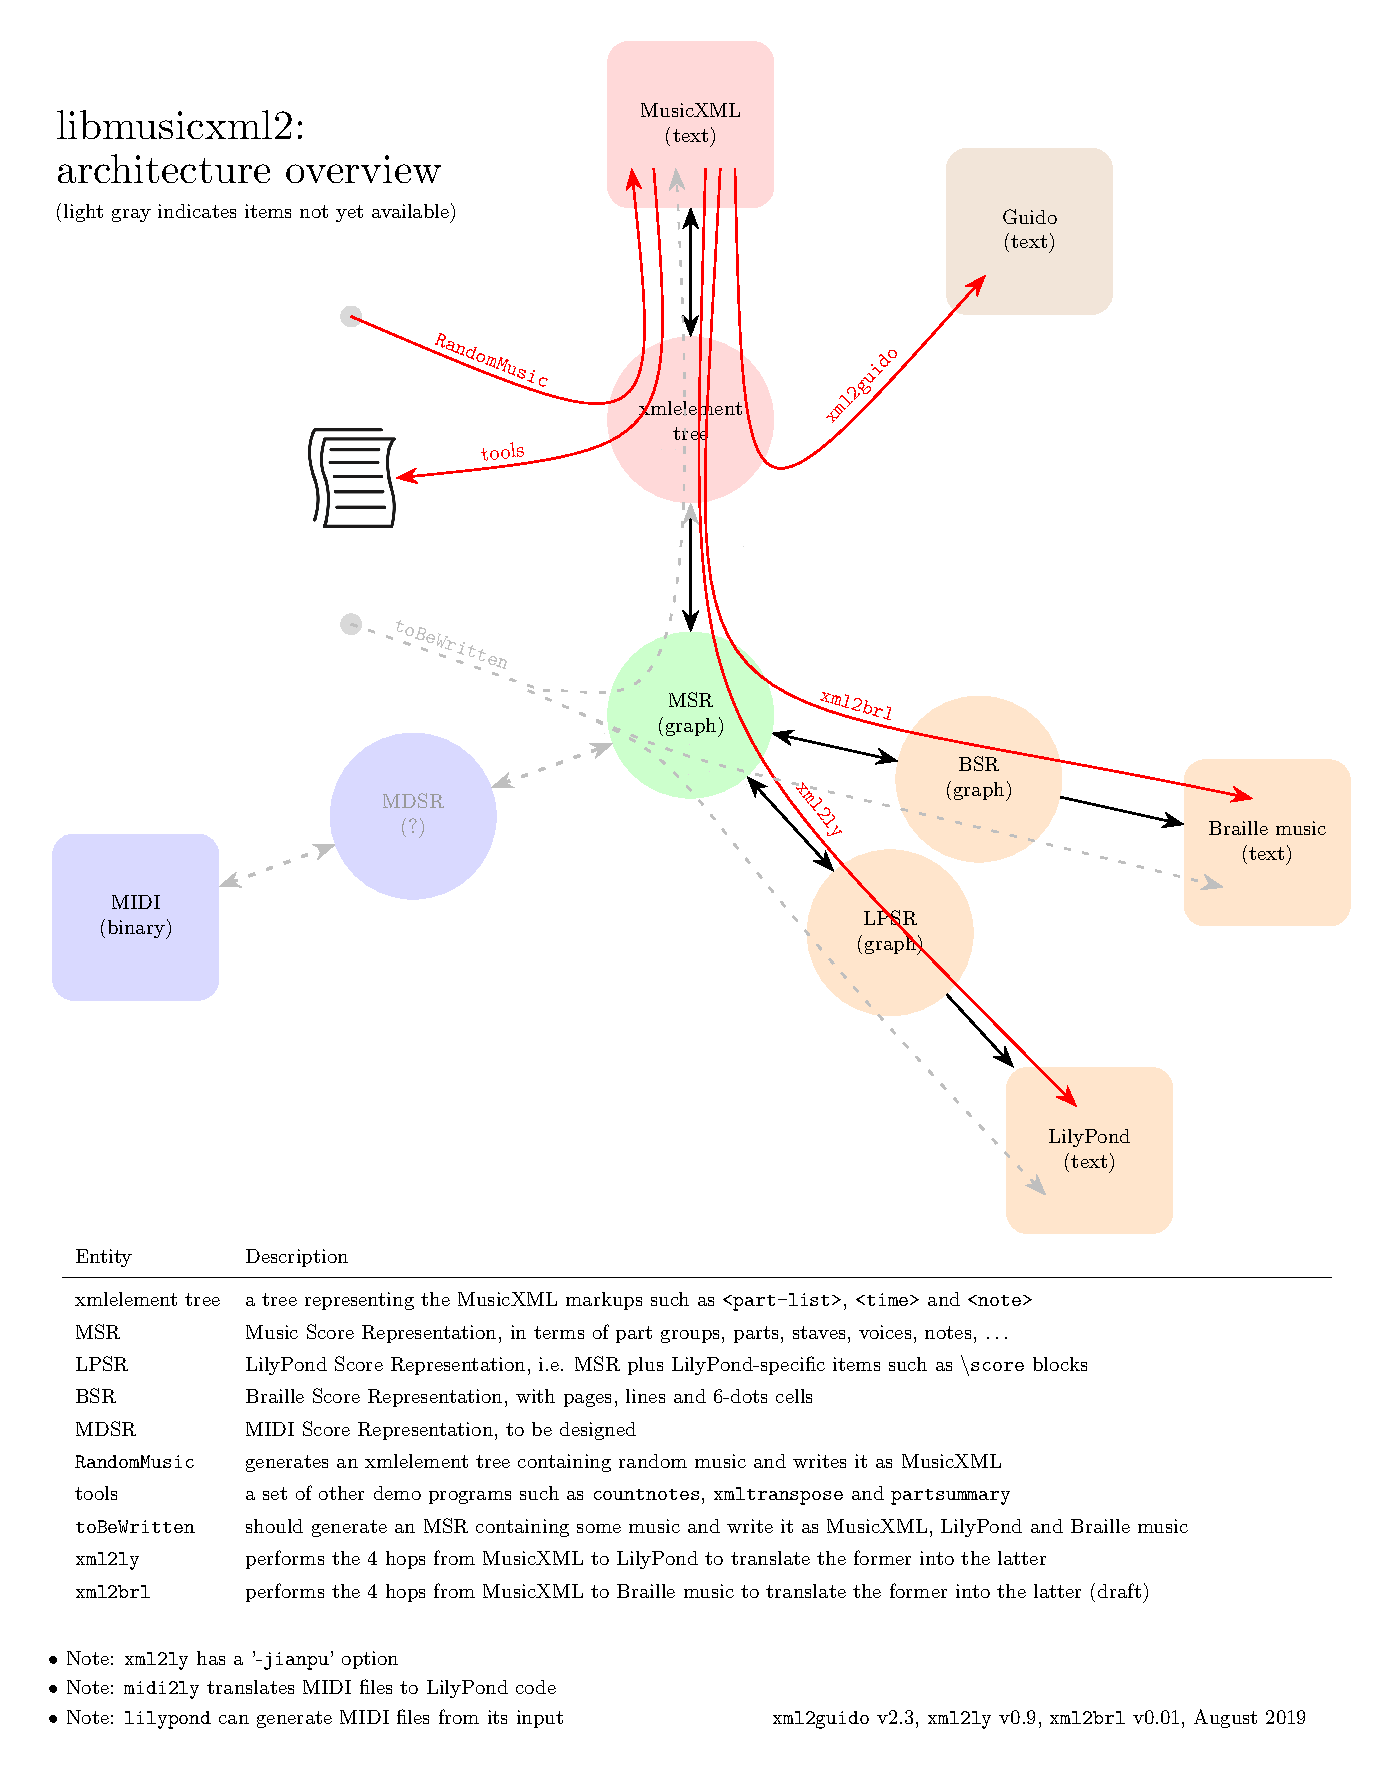
\includegraphics[scale=0.8]{../libmusicxmlArchitecture/libmusicxmlArchitecture.pdf}
\end{figure}


% -------------------------------------------------------------------------
% -------------------------------------------------------------------------
\section{Programming style and conventions}
% -------------------------------------------------------------------------
% -------------------------------------------------------------------------

The following text-editing conventions are used:
\begin{itemize}
\item tabs are not used before the first non-space character in a line, two spaces are used instead;

\item the code is not tightly packed: declarations in classes have the members' names aligned vertically, with many spaces before them if needed, and empty lines are used to separate successive activities in methods.
\end{itemize}

The code base of \xmlToLy\ is {\it defensive-programming} oriented, which means that:
\begin{itemize}
\item identifiers are explicit and long if needed -- only very local ones are short, such as iteration loops indexes;

\item the code is organized in sections, with an initial comment documenting what the code does.
\end{itemize}


% -------------------------------------------------------------------------
% -------------------------------------------------------------------------
% postamble
% -------------------------------------------------------------------------
% -------------------------------------------------------------------------

\pagebreak

\lstlistoflistings

%\listoffigures

\tableofcontents


% -------------------------------------------------------------------------
\end{document}
% -------------------------------------------------------------------------
